\documentclass[a4paper,10pt]{report}
\usepackage[francais]{babel}
\usepackage[utf8]{inputenc}
\usepackage{graphicx}
\usepackage{array}
\usepackage{caption}
\usepackage{subcaption}
\usepackage{float}
\newcommand{\HRule}{\rule{\linewidth}{0.5mm}}
\setcounter{secnumdepth}{3}
\setcounter{tocdepth}{3}

\date{2014-2015}

\begin{document}

\begin{titlepage}
 \begin{center}

 \begin{minipage}{0.4\textwidth}
    \begin{flushleft} \large
        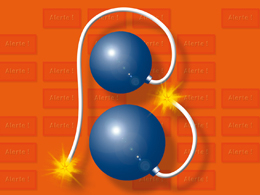
\includegraphics[width=3cm]{bonsai.jpg}
    \end{flushleft}
  \end{minipage}
  \begin{minipage}{0.4\textwidth}
    \begin{flushright} \large
      
\includegraphics[width=3cm]{lille1.png}
    \end{flushright}
  \end{minipage} 
  ~\\[3cm]

  \textsc{\LARGE PJI\\ Master 1 informatique}\\[1.5cm]

  \textsc{\Large Université Lille 1}\\[0.5cm]

  % Title
  \HRule \\[0.5 cm]
  { \huge \bfseries Prédiction de l'activité des peptides\\[0.8cm] \large \emph{CRISTAL - Equipe BONSAI} \\[0.4cm] }
  \HRule \\[1.5 cm]

  % Author and supervisor
  \begin{minipage}{0.4\textwidth}
    \begin{flushleft} \large
      \emph{Auteur:}\\
	Emilie \textsc{Allart}
    \end{flushleft}
  \end{minipage}
  \begin{minipage}{0.4\textwidth}
    \begin{flushright} \large
      \emph{Tuteurs:} \\
      Maude \textsc{Pupin} \\
      Laurent \textsc{Noé}
    \end{flushright}
  \end{minipage} 

  \\[3cm]
  {\large \emph{9 mars 2015} }
  \vfill
 \end{center}
\end{titlepage}


  \newpage
  \tableofcontents 
  \newpage

  \section*{Introduction}

      \paragraph
      \\
      ~~\\Au cours de la première année de master informatique, il est demandé d'effectuer un projet dans un laboratoire de recherche.
      J'ai donc effectué le mien au sein de l'équipe Bonsai, une équipe orientée bioinformatique faisant partie de CRISTAL. 
      Encadrée par Maude Pupin et Laurent Noé, j'ai travaillé sur le thème de : ' Rechercher les meilleurs critères pour la prédestination de l'activité d'un peptide'.
      Il s'agit donc d'analyser des peptides (petites protéines) dont nous connaissons déjà l'activité (antibiotique, anticancéreux, toxine, ...)  et de voir quelles informations sur elle auraient pu nous faire prédire son activité.
      Par exemple, ... TODO (chercher un exmeple pour illustrer)
      
      ~~\\Le but est de pouvoir par la suite, connaissant ces critères, prédire l'activité d'un peptide. Ainsi, nous pourrons trouver de nouvelles molécules avec des capacités thérapeutiques intéressantes, qui pourrait être synthétisées plus facilement. Trouver de nouveaux médicaments efficaces donc.
     
      ~~\\Pour ce faire, nous avons analysé les données de Norine (une base de données produites par l'équipe BONSAI).
      
      ~~\\Dans ce rapport, vous verrez donc le cahier des charges présantant le contexte et les différentes étapes à effectuer. Suivi de la mise en oeuvre, expliquant comment nous avons procédé. Et enfin les résulats seront traités.
      \addcontentsline{toc}{section}{Introduction}
      \newpage


  \chapter{Cahier des charges et contexte}

    ~~\\ Pour commencé posons les bases de notre réflexion ainsi que des outils utilisés.
    
    \section{Contexte}
      Comme dit précédemment le projet s'est déroulé au sein de l'équipe BONSAI, dans la branche portant sur les peptides non-ribosomiques (ou NRPs). Mais avant d'entrer dans la partie technique expliquons ce qu'est un NRP, ainsi que Norine.
      
      \subsection{NRPs}
	\paragraph{}
	  Tout d'abord un peptide, aussi appelé polymère, est constitués par des monomères . Relié entre eux par différentes liaisons, lui conférents des propriétés différentes. 
	  Un monomère ... 
	  TODO
	  
      \subsection{Norine}
	\paragraph{}
	  Norine est la première base de données entièrement dédiée aux peptides non ribosomiques.
	  TODO
    
	
      \subsection{Problématique}
	Détermination des meilleurs critères. 
	Pourquoi? 
	TODO
	
    \section{Cahier des charges}
	 
	 
	 \subsection{récupération des données}
	 
	    \paragraph{} 
	    Selon les différents critères nécessaires, nous relevons les données .. 
	    
	    
	 \subsection{Utilisation de weka}
	 
	    \paragraph{}
	    
	    Une fois les données récupérées, nous appliquons différentes méthodes d'apprentissage dessus.
	    Ainsi, nous pourrons convenir si les critères choisis apporte plus ou moins d'informations, et s'il est util de s'en servir pour prédire l'activité d'un peptide ou non. 
	    

	    \paragraph{Naive Bayes}
	    
	    ~\\Explication du principe de bayes
	    Exemple d'application: avec données, résultat, graph ...
	    
	    
	    \paragraph{SMO}
	    
	    ~\\idem 
	    
	    \paragraph{LibLinear}
	   
	    ~\\idem
	   
	 \subsection{Analyse des mesures de robustesse}
	     \paragraph{}
	     
	     Permet d'avoir la fiabilité de la prédiction
	     
	     \paragraph{Precision}
	      
	      ~\\
	      
	     
	     \paragraph{Sensibilité}
	     
	     \paragraph{F-measure}
	     
	     \paragraph{AUC ou ROC}
		
  
  \chapter{Mise en oeuvre}

  
    \section{Récupération depuis Norine}
    
	\paragraph{Les différents critères}
	    Surfactant, une activité, lien , composition
	    
   
    \section{Traitement des données}
	
	\paragraph{Comptage en monomère}
	    Prélèvement préalable des monomères.
	    Traitement de l'attribut composition de chaque peptide
	    Comptage pour chaque peptide de chaque occurence des monomères
	    Ajout au données
	    
	\paragraph{Comptage en cluster}
	    Prérequis : un fichier répertoriant les clusters de monomères.
	    cad un groupe de monomères auquel on assure qu'ils ont transmette une propriétés
	    Comptage pour chaque peptide du nombre d'occurence des élément d'un cluster pour chaque cluster.
	    Ajout aux données
	  
	\paragraph{Comptage en lien}
	    Traitement de l'attribut lien de chaque peptides
	    Comptage de lien (de 1 à 5) pour chaque peptides.
	    Ajout aux donnée
	
	\paragraph{Recupération au dessus d'un seuil}
	    Comptage du nombre de peptide ayant une certaine activité pour chaque activité.
	    Si le nombre de peptide possédant l'activité est inférieur au seuil, nous les enlevons de la base de données.
   
   
    \section{Choix des critères}
	  Comme vu précédemment, il est possible de faire différents traitements sur les données.
	  Ces traitements permettent de préparer les peptides pour voir si un critère apporte des connaissance sur ceuc-ci ou non.
	  Donc un critère dans le cadre de ce projet, peut être la quantité et l'apparition de monomères, de même pour les clusters, ou encore le possession d'un certain nombre de lien. 
	  
	  Une fois que les données seront traitées par le programme, sur différents critères, nous pourrons comparer leur utilitées en analysant la fiabilité de chaque prédiction
	 
     \section{Lancement des méthodes d'apprentissage}
	  
	  Une fois les données prêtes, il ne reste plus qu'à les analyser et voir si nous en tirons beaucoup d'information.
	  Pour ce fqire, nous avons utilisé 3 méthodes d'apprentissage comme cité précédement :
	  le naïveBayes, le SMO et le LibLinear. 
	  
	  Pour nous faire nous avons utiliser un wrapper weka permettant de continuer à travailler sur python.
	  Cependant, il a fallu installer une extension pour le LibLinear qui n'est pas implémenté de base. Pour se faire une librairie est ajoutée permettant de l'utiliser également.
	  
	  ce programme de lancement se décompose en fonction, chacune lancant une méthode, prenant en entrée le fichier contenant les données et donnant en sortie les mesures de robustesse à analyser.
	  
	  
     \section{mesures de robustesse}
	  
	  Nous obtenons ainsi un ensemble de mesures de robustesse qu'il faut comparer pour voir quel critère ou quel combinaison de critère est la plus efficace pour obtenir des informations sur un peptide.
	 
  \chapter{Résultats}

	  TODO : tableau comparatif
	  conclusion tirée de celui-ci
    
  \section*{Conclusion}
     
    \phantomsection
    \addcontentsline{toc}{section}{Conclusion}
    \newpage

    \newpage
    
    \section*{Glossaire}
    
    \phantomsection
    \addcontentsline{toc}{section}{Glossaire}
    \newpage

    \newpage
   
    \section*{Références}
     \end{itemize}

    \phantomsection
    \addcontentsline{toc}{section}{Annexe}
    \newpage

  \end{document}          
